图三显示了网络的两个数据连接层学习到的卷积核。该网络已经学习到了各种各样的频率与方向选择核,以及各种颜色点。注意两个GPU显示出的特性,3.5节中描述了一个结果是限制连接。GPU1上的核大部分颜色不明确,而GPU2上的核大多数颜色明确。这种特性在每一次运行中都会出现,且独立于所有特定的随机权重初始化(以GPU的重新编数为模)。\\ 

在图四的左边部分,通过计算该网络在八个测试图像上的top-5预测,我们可以定性的评估它到底学习到了什么。注意到即使是偏离中心的物体,比如左上角的一个小虫,也可以被网络识别到。大多数的top-5标签似乎是合理的。例如,对于美洲豹来说,只有其他类型的猫被认为是看似合理的标签。在某些情况下(铁栅、樱桃),对于图片意图的焦点存在歧义。\\

\begin{figure}[h]
  \centering
  \scalebox{0.6}{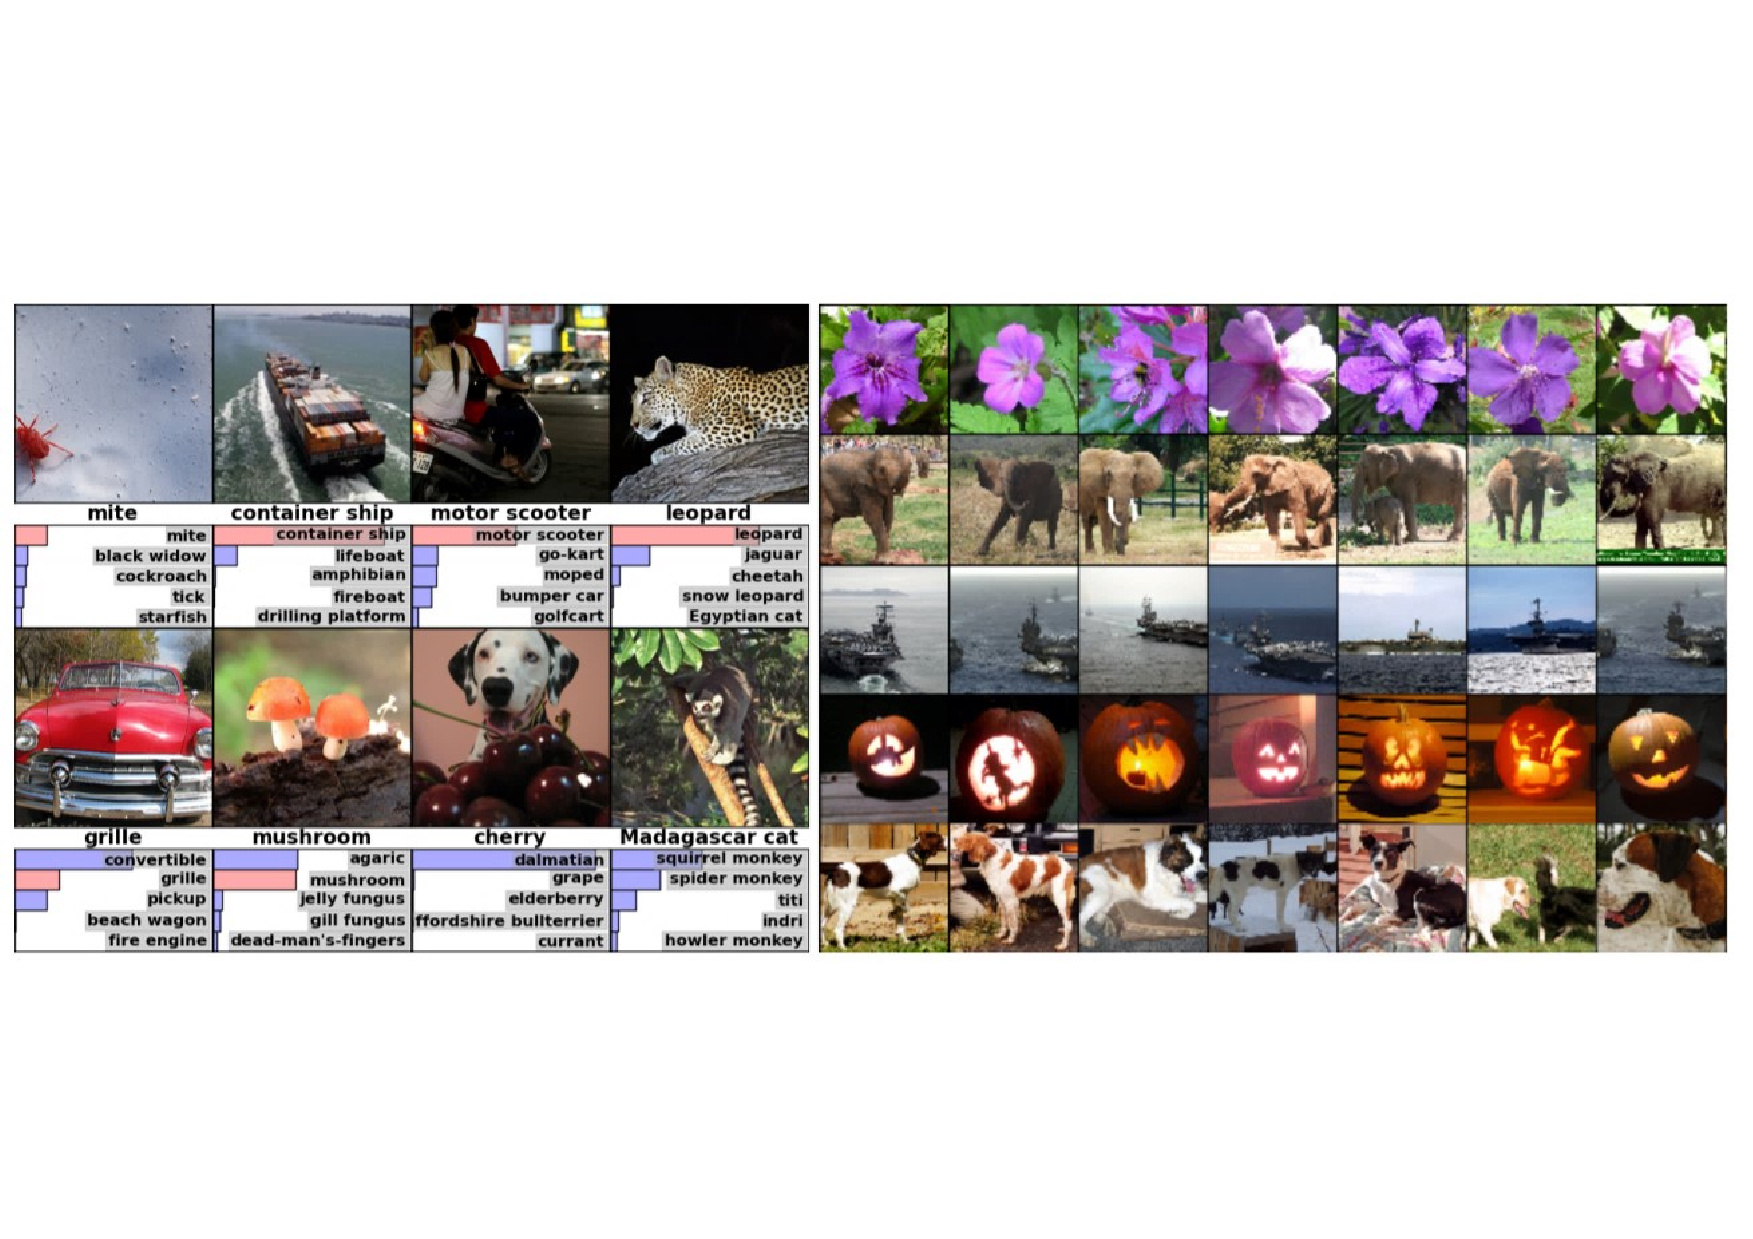
\includegraphics{4.pdf}}
  \caption{(左)8张ILSVRC-2010测试图像和我们的模型认为最可能的5个标签。每张图像的下面是它的正确标签,正确标签的概率用红条表示(如果正确标签在前五当中)。(右)第一列是5张ILSVRC-2010测试图像。剩下的列展示了6张训练图像,这些图像的最后的隐藏层的特征向量与测试图像的特征向量有最小的欧氏距离。}
  \label{fig:fig4}
\end{figure}

另外一个探索网络可视化知识的方法是考虑最后4096维隐藏层在图像上得到的特征激活。如果两幅图像生产的特征激活向量之间有较小的欧氏距离,我们可以说,在神经网络更高级别上认为它们是相似的。图四展示了测试集中的五个图像,以及训练集中根据这一标准与其中每一个最相似的六个图像。注意,在像素级别,检索到的训练图像一般不会接近第一列中的查询图像。例如,检索到的狗和大象表现出各种各样的姿势。我们会在补充材料里给出更多测试图像的结果。\\

通过使用两个4096维实值向量间的欧氏距离来计算相似性是效率低下的,但它可以通过训练一个自编码器将这些向量压缩为短的二进制代码来变得高效。这应该会产生一个比将自编码器直接应用到原始图像上好得多的图像检索方法[14],它不利用图像标签,因此会趋向于检索与要检索的图像具有相似边缘模式的图像,而不论它们在语义上是否相似。\\
